
\documentclass{article}
\usepackage{graphicx}
\usepackage{algorithm}
\usepackage{algpseudocode}
\usepackage{float}

\usepackage[utf8]{inputenc}
\usepackage[english]{babel}
\setlength{\parindent}{0em}
\setlength{\parskip}{1em}

\usepackage{geometry}


\geometry{
a4paper,
total={170mm,257mm},
left=20mm,
top=20mm,
}


\usepackage{listings}

\usepackage{amsmath}
\DeclareMathOperator{\arcsec}{arcsec}


\begin{document}

\title{Laplace}

\author{2081052,2089602,2073835,2072566, 2091324}


\date{\today}

\maketitle


\begin{abstract}

\end{abstract}


\section{Introduction}

\subsection{Systems}
The project focused on three systems:

System 1 is two concentrical cylinders. The inner cylinder is kept at groud potential and the outer cylinder is kept at a postive potential. This is shown in Figure  \ref{fig:System1}.

\begin{figure}[H]
\centering
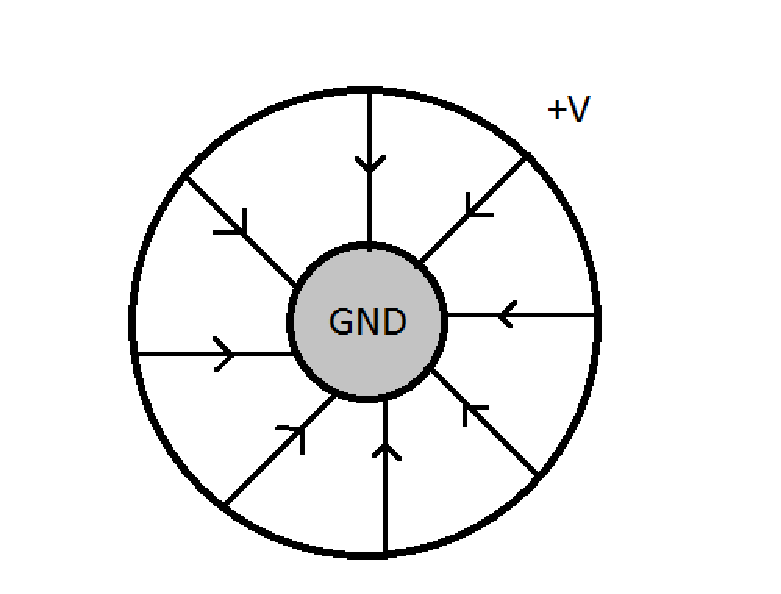
\includegraphics[width=75mm]{System1.pdf}
\caption{Diagram of system 1}
\label{fig:System1}
\end{figure}

System 2 has two parallel infinite plates, one at positive V and one at negative V, with a cylinder in the centre kept at ground potential. This is shown in Figure \ref{fig:System2}
 
\begin{figure}[H]
\centering
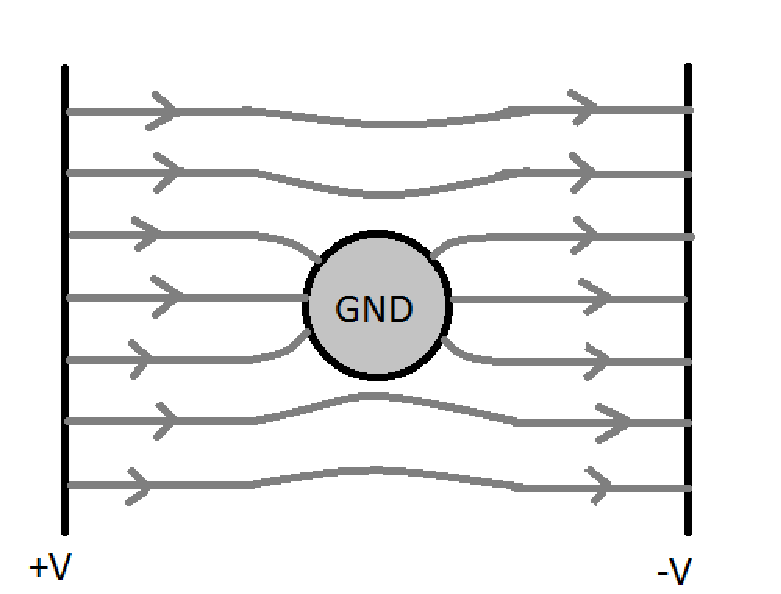
\includegraphics[width=75mm]{System2.pdf}
\caption{Diagram of system 2}
\label{fig:System2}
\end{figure}

Both Systems 1 and 2 can be solved both analytically and numerically. System 1 has an exact analytical solution but System 2 requires some approximations to obtain an analytical solution.

The third system was a Silicon Microstrip Detector.

\begin{figure}[H]
\centering
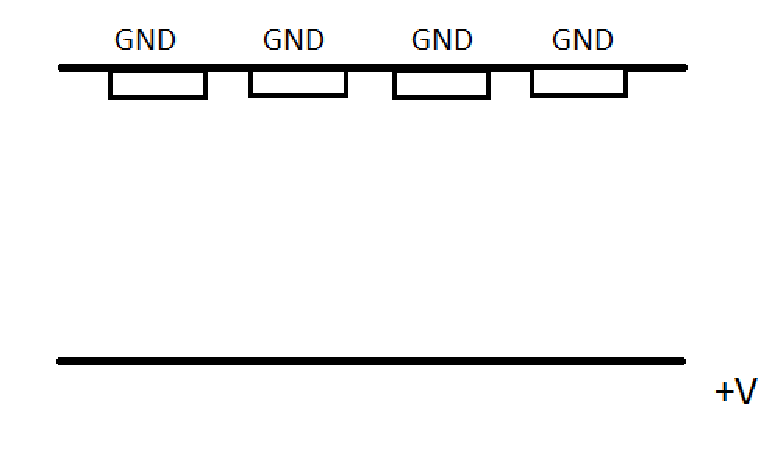
\includegraphics[width=75mm]{Silicon.pdf}
\caption{Diagram of Silicon system}
\label{fig:Silicon}
\end{figure}

Figure \ref{fig:Silicon} shows implants kept at ground potential and a backplane kept at positive V. This system cannot be solved analytically and can only be solved numerically.


\section{Analytical Solution}



\section{Numerical Solution}


\subsection{Methods}



It is not always possible to find an analytical solution as in real world
situations the boundary conditions are not infinite. This means the systems
need to be solved numerically and this is done using the finite difference
method.These can be derived from Laplace's equation:

\begin{equation}\bigtriangledown ^{2}\varphi =\frac{\partial ^{2}\varphi }{\partial x^{2}} + \frac{\partial ^{2}\varphi }{\partial y^{2}}=0 \end{equation}

The Laplace's equation is an elliptic partial differential equation. It can be used to solve problems in electrostatics, fluid potentials and is the steady state heat equation.

To obtain the finite difference method a square lattice with length d and grid spacing h is needed. Each point is labelled and an arbitrary point $\Phi_{i,i}$ is taken. The Taylor Series expansions of the four points surrounding the arbitrary centre point are calculated.

\begin{equation} \Phi_{i+1,j} = \Phi_{i,j} + \Delta x \frac{\partial \Phi_{i,j}}{\partial x } + \frac{\Delta x^{2}}{2}\frac{\partial^{2}\Phi_{i,j}}{\partial x^{2}}
\end{equation}

These expansions are then used to approximate $\frac{\partial^{2}\Phi_{i,j}}{\partial x^{2}}$ and $\frac{\partial^{2}\Phi_{i,j}}{\partial y^{2}}$ to obtain the finite difference method:

\begin{equation} \frac{\Phi_{i+1,j}-2\Phi_{i,j}+\Phi_{i-1,j} }{\Delta x^{2}}+\frac{\Phi_{i,j+1}-2\Phi_{i,j}+\Phi_{i,j+1} }{\Delta y^{2}} \end{equation}


The simplest method using the finite difference method is the Jacobi's Iterative method.However, this method takes more iterations, i.e. more computing time, for the numerical answer to equalthe analytical solution.


\begin{equation} U_{n+1,j,k}=\frac{1}{4}\left[ U_{n,j+1,k} + U_{n,j-1,k} + U_{n,j,k+1} +U_{n,j,k-1}\right]
\end{equation}

Another method which is quicker is the Gauss-Seidel method. Unlike the Jacobi method it does not store the previous values and uses the points that have already been 'updated' to caluclate the next value.

\begin{equation} 
U_{n+1,j,k}=\frac{1}{4}\left[ U_{n,j+1,k} + U_{n+1,j-1,k} + U_{n,j,k+1} +U_{n+1,j,k-1}\right]
\end{equation}

The Successive Over Relaxation (SOR) method uses both the new and old solutions in a linear combination.

\begin{equation} 
U_{n+1,j,k}=\left(1-\omega\right). U_{n,j,k}+\frac{\omega}{4}\left [ U_{n,j+1,k} + U_{n+1,j-1,k} + U_{n,j,k+1} +U_{n+1,j,k-1}\right]
\end{equation}


The $\omega$ is the over-relaxation parameter and this can be changed to optimize the results. For a square lattice the SOR method converges fastest if:


\begin{equation}
\omega \simeq \frac{2}{1 + \frac{\pi}{d}}
\end{equation}

where d is the number of grid points in either direction. \cite{numericalmethods}

\subsection{Method Comparison}

The different numerical methods were compared for System 2. The methods were compared for the following setup on the initial codes. Plates at voltage 10, distance 100, height 100, circle of radius 15 amd acceptable precision 0.001.



The Jacobi method took 1514 iterations. This took a computing time of 0.94s.


The Gauss-Seidel method took 962 iterations. This took a computing time of 0.73s.


The SOR method took 165 iterations. This took a computing time of 0.28s.




It can clearly be seen that the best method is the SOR method.


The following graph shows the rate of convergence of all three methods.




For the general solver the following setup was used to obtain the following results. Plates at voltage 5 and -5, distance and height 100, radius 10 and acceptable precision 0.001.


The Jacobi method took 1113 iterations and 3.08s.




The Gauss-Seidel method took 822 iterations and 2.3s.


The SOR method took 496 iterations and 1.69s.




\section{Programming and Technical Challenges}
The goal was to produce a program that would allow the user to input any set of boundary conditions, and then run one of the three finite difference methods discussed above repeatedly until further iterations of the method made no change. Then the program should somehow plot the resulting electric and potential fields.

\subsection{The \texttt{grid} variable}
The first problem was to choose a suitable data type to represent the space being investigated. As in any numerical approximation, the continuous space must be divided into a very large number of discrete cells, each representing a point in space. The data structure that was chosen is as follows: \texttt{vector<vector<tuple<double,bool>>>}. This is a 2-dimensional \texttt{vector}, with \texttt{tuple}s as entries, representing the cells.

The position on the first \texttt{vector} represents the cell's x-coordinate, and the position on the second its y-coordinate. The first entry in the tuple representing the cell is a \texttt{double} value representing the potential at that point, and the second entry is a \texttt{bool} value indicating whether that cell is part of the boundary conditions (true), or not (false). If the cell is part of the boundary conditions, it must never be changed during the operation of the finite difference methods.
\subsection{The \texttt{Board} class}
On a higher level, spaces being investigated are represented by members of a class called \texttt{Board}. This class has \textbf{two} of the above data types as variables, called \texttt{grid} and \texttt{new\_grid}. These represent the information about the space before and after the most recent iteration of the chosen finite difference method. The class also has member functions which allow the important operations to be carried out on the board. These functions will be discussed in the order in which they are used by the program.

\subsubsection{Initialisation}
A major challenge in the development of the program was to find a way to allow the user to input arbitrary boundary conditions, in a relatively user-friendly way. The solution that was decided upon is to take input in the form of a Bitmap file. When the function \texttt{bmpInitialise(bmp\_filename)} is called, each pixel in the input Bitmap file is mapped to the corresponding cell in \texttt{grid} and \texttt{new\_grid}. The colour of the pixel is detected. If the pixel is pure red (RGB = 255,0,0), the potential of its corresponding cell is set to +5V, and its boolean is set to true. Similarly, if the pixel is pure green, its potential is set to 0V, and if the pixel is pure blue it is set to -5V. In this manner, the values of \texttt{grid} and \texttt{new\_grid} may be initialised to represent any arrangement of charged plates, cylinders, or any other two-dimensional shape the user chooses.

%INSERT EXPLANATORY GRAPHIC

\subsubsection{Iteration}
The next problem was to write methods that perform single iterations of each of the finite difference methods described in Section 3.1. For the most part this was a simple matter of expressing the equations described in that section in C++ code. However, one technical problem worth commenting on is that of the edge cases. Since the finite difference methods are based on finding the average of neighbouring cells, great care must be taken when finding the next value of the potential for cells on the edge or corner of the grid, since in these cases we must explicitly state that we are looking for the average of, say, the cell to the left of and the cell above in the case of the cell on the bottom-right corner of the grid. Each time one of the finite difference methods is called, it begins by setting \texttt{grid} equal to \texttt{new\_grid}, and updates only \texttt{new\_grid}, so they remain one iteration apart.


\subsubsection{Convergence}
The program should run for only as long as it is doing useful operations. Therefore a function is required that detects when further iterations of the finite difference methods are producing no change in the values of the potential in each cell. This is why we store both \texttt{grid} and \texttt{new\_grid}, rather than just one. We need to be able to compare the current values with the values before the most recent iteration. The function \texttt{converged(precision)} returns true if the difference between the potential in every cell in \texttt{new\_grid} and the potential in the corresponding cell in \texttt{grid} is less than the provided precision value.

\subsubsection{Output}
The function \texttt{writeBoard(output\_filename)} takes the current value of \texttt{new\_grid} and writes it to a three-column data file in the format

%X-COORD        Y-COORD     POTENTIAL

It also writes a second text file that contains the gradient of the potential in both the x and y directions.

X- COORD                    Y-COORD          X GRADIENT          Y-GRADIENT

\subsection{Electric field graph}

The electric field is the negative gradient of the electric potential:

\begin{equation} E=-\bigtriangledown V \end{equation}

These two files created by the general solver are used to create an electric field graph. Gnuplot is used to plot this graph.

The text files containing the potentials is plotted using splot (the 3d plotting tool in gnuplot) with a contour base set. On top of this the text files containing the gradients is plotted with vectors. This produces a graph like the following:


This was produced from the following bitmap:




\subsection{Program Structure}
The overall structure of the C++ program is shown below:

% INSERT UML DIAGRAM

As discussed above, the \texttt{Board} class contains most of the important functions. The actual running of the program is managed in the \texttt{Source} file, which asks the user for input regarding which finite difference method to use, and the desired accuracy level, and creates instances of \texttt{Board} and runs the member functions with appropriate parameters.

% Describe Bash script here.

\section{Example Application: Silicon Microstrip Detector}
As a demonstration of the capabilities of this program, we present its application to an important physical situation. Silicon microstrip detectors consist of a positively charged 'backplane' opposite a large number of grounded silicon wafers, as shown below:

% Insert SMD graphic

These are often used to detect ionising radiation in particle physics experiments. Therefore it is very important to understand the electric field around such arrangements of charge. The first step is to create a Bitmap file representing the situation. Such an image is shown below:

\begin{figure}[H]
\centering
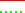
\includegraphics[width=50mm]{silbitmap.pdf}
\caption{Bitmap of Silicon system}
\label{fig:bitmapsilicon}
\end{figure}

When this file is provided as an argument to the Bash script, the resulting plots for the potential and electric fields are shown below:

\begin{figure}[H]
\centering
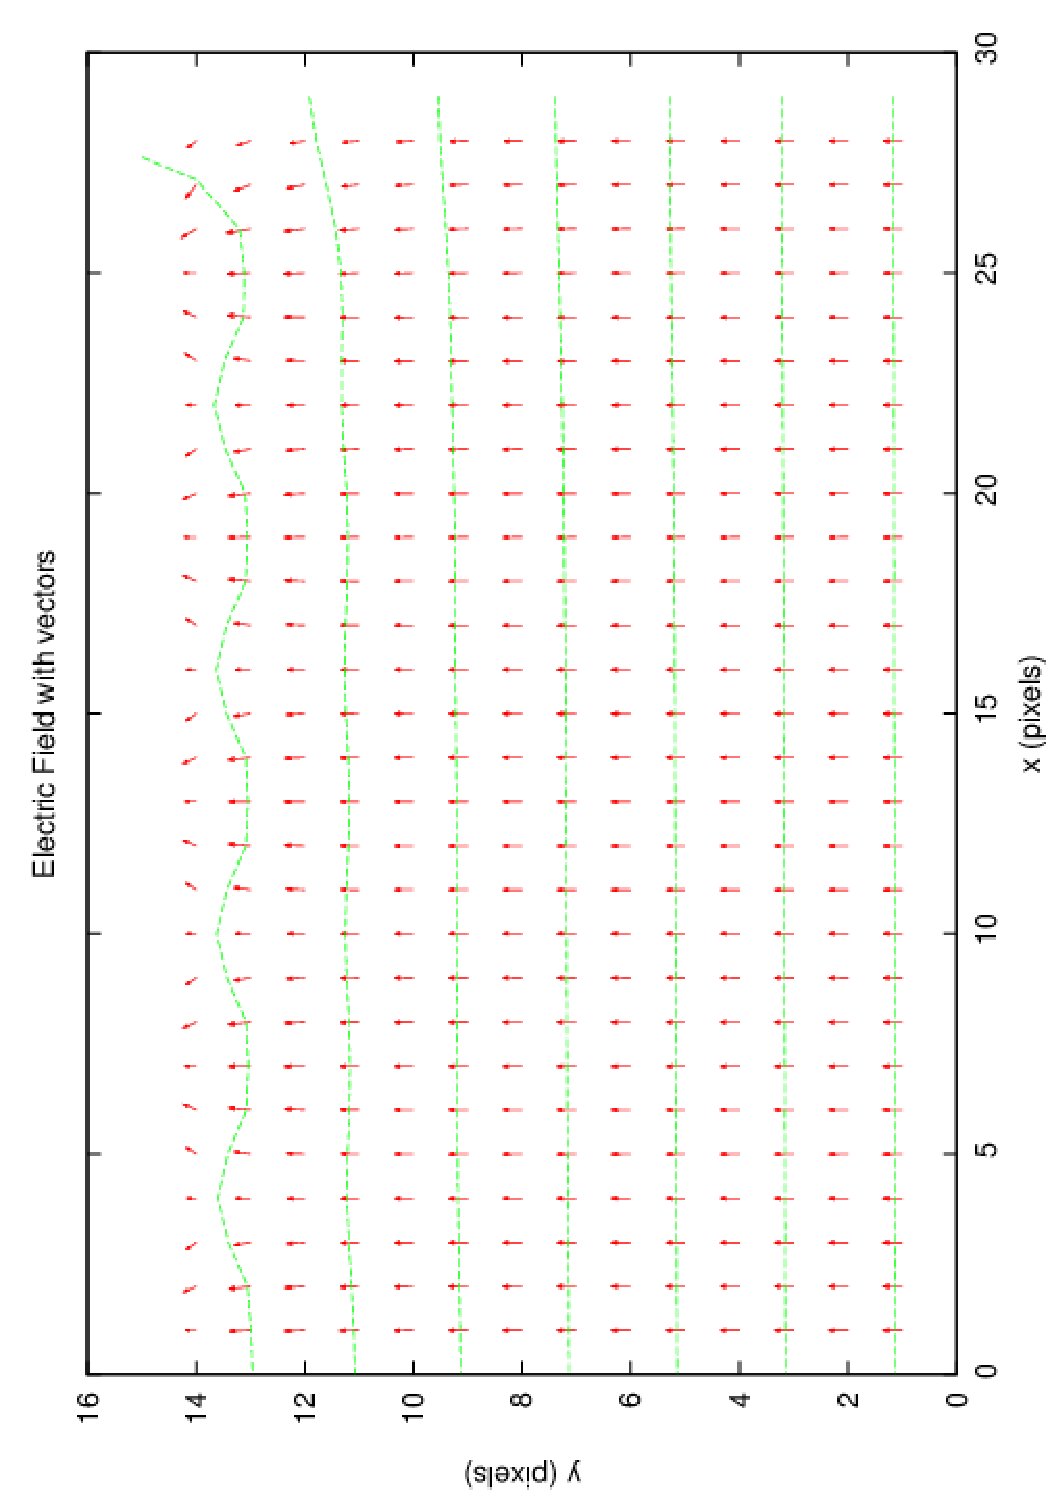
\includegraphics[width=50mm,angle=270]{siliconelec.pdf}
\caption{Electric Field diagram of Silicon system}
\label{fig:siliconelec}
\end{figure}









\section{Conclusion}












\section{Appendix}


\subsection{Algorithm of SOR method for System 2}


\begin{algorithm}


\begin{algorithmic}


\Procedure {The SOR method}{}


\State Initialise Variables


\State V - Potential on plates


\State d - Distance between plates


\State h - Height of plates


\State r- Radius of inner circle


\State error - Acceptable prescision


\State errorcount - Count error


\State omega =$ 2/(1+ \pi/d)$ - Relaxation parameter


\State dx, dy - Grid spacing


\State xstep = d/dx;


\State ystep = h/dy;


\State u[xstep +2][ystep +2] - Multidimensional array for potential


\State unew[xstep +2][ystep + 2] - Multidimensional array for updated potential


\State Boundary Conditions:


\For {int j=0; j$<$xstep; j++}


\For {int k=0; k$<$ystep;k++}


\If {j==0 $||$ j==xstep}


\State u[j][k]=V;


\State unew[j][k]=u[j][k];


\ElsIf{k==0 $||$ k==ystep}


\State u[j][k]=$V-(2*V*j)/xstep$;


\State unew[j][k]=u[j][k];


\Else


\State u[j][k]=0;


\State unew[j][k]=u[j][k];


\EndIf


\EndFor


\EndFor


\State SOR method:


\While {errorcount <xstep -1}


\State errorcount =0;


\For{int j=1;j$<$xstep;j++}


\For {int k=1;k$<$ystep;k++}


\If {Inside Ground Circle}


\State unew[j][k]=0;


\Else


\State unew[j][k]=$(1-omega)*u[j][k]+(0.25)*(omega)*(unew[j-1][k]+u[j+1][k] + unew[j][k-1] + u[j][k+1]$;


\EndIf


\EndFor


\EndFor


\For {int j=0; j$<$xstep; j++}


\If {Convergence$<$error}


\State errorcount+=1;


\EndIf


\EndFor


\For {int j=1; j$<$(xstep); j++}


\For {int k=1;k$<$(ystep);k++}


\State u[j][k]=unew[j][k];


\EndFor


\EndFor


\EndWhile


\caption{SOR method Algorithm}


\EndProcedure


\end{algorithmic}


\end{algorithm}












\begin{thebibliography}{9}







\bibitem{numericalmethods}


Richard J. Gonsalves . 2011. \textit{Poisson's Equation and Relaxation Methods.} [ONLINE] Available at: http://www.physics.buffalo.edu/phy410-505/2011/topic3/app1/index.html. [Accessed 11 February 16]


    


\end{thebibliography}


.







\end{document}

